PyMC probability models are linked collections of nodes. These nodes are only informed by the value of their parents. \code{Deterministic} instances can compute their values given their parents' values, \code{Stochastic} instances can compute their log-probabilities or draw new values, and \code{Potential} instances can compute their log-probabilities. Fitting probability models requires larger-scale coordination and communication.

All objects capable of fitting probability models are subclasses of the \code{Model} class. All objects that fit probability models using some kind of Monte Carlo method are descended from the \code{Model} subclass \code{Sampler}. \code{Sampler} provides a generic sampling loop method and database support for storing large sets of joint samples. %Sampling loops can optionally be run interactively, meaning the user can pause sampling at any time, return to the Python prompt, check progress, and make adjustments.

PyMC provides three Sampler subclasses for fitting models:
\begin{itemize}
    \item \code{MCMC}, which coordinates Markov chain Monte Carlo algorithms. The actual work of updating stochastic variables conditional on the rest of the model is done by \code{StepMethod} instances, which are described in this chapter.
    \item \code{MAP}, which computes maximum \emph{a posteriori} estimates.
    \item \code{NormApprox}, which computes the `normal approximation' \cite{gelman}: the joint distribution of all stochastic variables in a model is approximated as normal using local information at the maximum \emph{a posteriori} estimate.
\end{itemize}

\hypertarget{model}{}
\section*{The \code{Model} class} \label{sec:Model}
\pdfbookmark[1]{The Model class}{model}
This class serves as a container for probability models and as a base class for the classes responsible for model fitting, such as \code{MCMC}.

Models' useful methods are:
\begin{description}
    \item[\code{draw_from_prior()}:] Sets all stochastic variables' values to new random values, which would be a sample from the joint distribution if all data and \code{Potential} instances' log-probability attributes were set to zero. If no \code{random()} method exists, PyMC will raise an exception.
    \item[\code{seed()}:] Same as \code{draw_from_prior}, but only \code{stochastics} whose \code{rseed} attribute is not \code{None} are changed.
    \item[\code{find_generations():}] Sets the \code{generations} attribute. This attribute is a list whose elements are sets of stochastic variables. The zeroth set has no extended parents in the model, the first set only has extended parents in the zeroth set, and so on.
\end{description}

The helper functions \code{weight} and \code{graph} act on models. \code{weight} computes Bayes' factors (posterior probabilities of model correctness) for lists of models using the \code{draw_from_prior} method, and \code{graph} produces graphical representations \cite[see]{Jordan:2004p5439}. The \code{weight} function's algorithm can only be expected to perform well when the dimension of the parameter space is small (less than about 10).

Models have the following important attributes:
\begin{itemize}
    \item \code{variables}
    \item \code{stochastics}
    \item \code{potentials}
    \item \code{deterministics}
    \item \code{data_stochastics}
    \item \code{step_methods}
    \item \code{value}
\end{itemize}

In addition, models expose each node they contain as an attribute. For instance, if model \code{M} were produced from model (\ref{disastermodel}) \code{M.s} would return the switchpoint variable. It's a good idea to give each variable a unique name if you want to access them this way.


\subsection*{Creation of models} \label{sec:ModelInstantiation}
The \code{Model} class's init method takes the following arguments:
\begin{description}
    \item[\code{input}:] Some collection of PyMC nodes defining a probability model. These may be stored in a list, set, tuple, dictionary, array, module, or any object with a \code{__dict__} attribute. If \code{input} is \code{None} (the default), all the nodes on the main namespace and the \code{Model} object's class's dictionary are collected.
    \item[\code{verbose} (optional):] An integer controlling the verbosity of the model's output.
\end{description}
The \code{input} argument can be just about anything; once you have defined the nodes that make up your model, you shouldn't even have to think about how to wrap them in a \code{Model} instance. Some examples of model instantiation, using nodes \code{a}, \code{b} and \code{c}:
\begin{itemize}
    %\item \code{M = Model(a,b,c)} THIS ONE DOES NOT WORK -- JUST TRIED IT
    \item \code{M = Model(set([a,b,c]))}
    \item \code{M = Model(\{`a': a, `d': [b,c]\})}
    \item \code{M = Model([[a,b],c])}
    \item File \code{MyModule} containing the definitions of \code{a}, \code{b} and \code{c}:\begin{verbatim}
import MyModule
M = Model(MyModule)
    \end{verbatim}
    \item `Model factory' function:
    \begin{verbatim}
def make_model(x):
    a = Exponential('a',.5,beta=x)
    
    @deterministic
    def b(a=a):
        return 100-a
    
    @stochastic
    def c(value=.5, a=a, b=b);
        return (value-a)**2/b
        
    return locals()
    
M = Model(make_model(3))
    \end{verbatim}
    \item Model subclasses are inspected for nodes:
    \begin{verbatim}
class MyModel(Model):
    a = Exponential('a',.5,beta=x)

    @deterministic
    def b(a=a):
        return 100-a

    @stochastic
    def c(value=.5, a=a, b=b);
        return (value-a)**2/b        
        
M = MyModel()
    \end{verbatim}    
    \item If no input argument is provided, the main namespace is inspected for nodes:
    \begin{verbatim}
    a = Exponential('a',.5,beta=x)

    @deterministic
    def b(a=a):
        return 100-a

    @stochastic
    def c(value=.5, a=a, b=b);
        return (value-a)**2/b        
    
    M = Model()
    \end{verbatim}

\end{itemize}

\hypertarget{sampler}{}
\section*{The \code{Sampler} class} \label{sec:Sampler}
\pdfbookmark[1]{The Sampler class}{sampler}
Samplers fit models with Monte Carlo fitting methods, which characterize the posterior distribution by approximate samples from it. They are initialized as follows: \code{Sampler(input=None, db='ram', name='Sampler', reinit_model=True, calc_deviance=False)}. The \code{input} argument is a module, list, tuple, dictionary, set, or object that contains all elements of the model, the \code{db} argument indicates which database backend should be used to store the samples (see chapter \ref{chap:database}), \code{reinit\_model} is a boolean flag that indicates whether the model should be re-initialised before running, and \code{calc\_deviance} is a boolean flag indicating whether deviance should be calculated for the model at each iteration. Samplers have the following important methods:
\begin{description}
    \item[\code{sample(iter, length=None, verbose=0)}:] Samples from the joint distribution. The \code{iter} argument controls how many times the sampling loop will be run, and the \code{length} argument controls the initial size of the database that will be used to store the samples.
    \item[\code{isample(iter, length=None, verbose=0)}:] The same as \code{sample}, but the sampling is done interactively: you can pause sampling at any point and be returned to the Python prompt to inspect progress and adjust fitting parameters. While sampling is paused, the following methods are useful: 
    \begin{description}
        \item[\code{icontinue()}:] Continue interactive sampling.
        \item[\code{halt()}:] Truncate the database and clean up.
    \end{description}
    \item[\code{tally()}:] Write all variables' current values to the database. The actual write operation depends on the specified database backend.
    %\item[\code{draw()}:] Not currently used. In future Monte Carlo fitting methods that aren't MCMC, such as importance samplers, the \code{draw()} method will be responsible for drawing approximate samples from the joint distribution (by setting the values of all the stochastic variables in the model).
    \item[\code{save\_state()}:] Saves the current state of the sampler, including all stochastics, to the database. This allows the sampler to be reconstituted at a later time to resume sampling. This is not supported yet for the RDBMS backends, sqlite and mysql.
    \item[\code{restore\_state()}:] Restores the sampler to the state stored in the database.
	 \item[\code{stats()}:] Generate summary statistics for all nodes in the model.
    \item[\code{remember(trace\_index)}:] Set all variables' values from frame \code{trace\_index} in the database. Note that the \code{trace_index} is different from the current iteration, since not all samples are necessarily saved due to burning and thinning. 
\end{description}

In addition, the sampler attribute \code{deviance} is a deterministic variable valued as the model's deviance at its current state.

\hypertarget{MAP}{}
\section*{Maximum a posteriori estimates} \label{sec:MAP}
\pdfbookmark[1]{Maximum a posteriori estimates}{model}

The \code{MAP} class sets all stochastic variables to their maximum a posteriori values using functions in SciPy's \code{optimize} package. SciPy must be installed to use it. A \code{MAP} instance \code{M} can be created as follows:
\begin{verbatim}
M = MAP(input, eps=.001, diff_order = 5)    
\end{verbatim}
The parameters \code{eps} and \code{diff_order} control numerical differentiation. \code{diff_order}, which must be an integer, specifies the order of the numerical approximation (see the SciPy function \code{derivative}). The step size for numerical derivatives is controlled by \code{eps}, which may be either a single value or a dictionary of values whose keys are variables (actual objects, not names). \code{MAP} requires all stochastic variables in \code{input} to be either float-valued or array-valued with dtype float, unlike PyMC in general.

\code{MAP} has two useful methods:
\begin{description}
    \item[\code{fit(method ='fmin', iterlim=1000, tol=.0001)}:] The optimization method may be \code{fmin}, \code{fmin_l_bfgs_b}, \code{fmin_ncg}, \code{fmin_cg}, or \code{fmin_powell}. See the documentation of SciPy's optimize package for the details of these methods. The \code{tol} and \code{iterlim} parameters are passed to the optimization function under the appropriate names.
    \item[\code{revert_to_max()}:] If the values of the constituent stochastic variables change after fitting, this function will reset them to their maximum a posteriori values.
\end{description}

The useful attributes of \code{MAP} are:
\begin{description}
    \item[\code{logp}:] The joint log-probability of the model.
    \item[\code{logp_at_max}:] The maximum joint log-probability of the model.
    \item[\code{len}:] The total number of elements in all the stochastic variables in the model with \code{observed=False}.
    \item[\code{data_len}:] The total number number of elements in all the stochastic variables in the model with \code{observed=True}.
    \item[\code{AIC}:] Akaike's information criterion for this model \cite{Akaike:1973aj,Burnham:2002ic}.
    \item[\code{BIC}:] The Bayesian information criterion for this model \cite{Schwarz:1978ud}.
\end{description}

One use of the \code{MAP} class is finding reasonable initial states for MCMC chains. Note that multiple \code{Model} subclasses can handle the same collection of nodes.

\hypertarget{norm-approx}{}
\section*{Normal approximations} \label{sec:norm-approx}
\pdfbookmark[1]{Normal approximations}{norm-approx}

The \code{NormApprox} class extends the \code{MAP} class by approximating the posterior covariance of the model using the Fisher information matrix, or the Hessian of the joint log probability at the maximum. In addition to the methods and attributes of \code{MAP}, it provides the following methods inherited from \code{Sampler}:
\begin{description}
    \item[\code{sample(iter)}:] Samples from the approximate posterior distribution are drawn and stored.
    \item[\code{isample(iter)}:] An `interactive' version of \code{sample()}: sampling can be paused, returning control to the user.
\end{description}
It provides the following additional attributes:
\begin{description}
    \item[mu:] A special dictionary-like object that can be keyed with multiple variables. \code{N.mu[p1, p2, p3]} would return the approximate posterior mean values of stochastic variables \code{p1}, \code{p2} and \code{p3}, ravelled and concatenated to form a vector.
    \item[C:] Another special dictionary-like object. \code{N.C[p1, p2, p3]} would return the approximate posterior covariance matrix of stochastic variables \code{p1}, \code{p2} and \code{p3}. As with \code{mu}, these variables' values are ravelled and concatenated before their covariance matrix is constructed.
\end{description}

\hypertarget{mcmc}{}
\section*{Markov chain Monte Carlo: the \code{MCMC} class} \label{sec:mcmc}
\pdfbookmark[1]{The MCMC class}{mcmc}
 \code{MCMC} is a subclass of \code{Sampler}. At the beginning of a sampling loop, it assigns a \code{StepMethod} instance (section \ref{sec:stepmethod}) to each stochastic variable for which the user has not created one. Step methods are assigned as follows: each \code{StepMethod} subclass in existence is allowed to inspect the variable in question and determine its competence to handle the variable, on a scale of 0 to 3. An instance of the highest bidder is created to handle the variable.

MCMC samplers have the following methods, in addition to those of \code{Sampler}:
\begin{description}
    \item[\code{sample(iter, burn=0, thin=1, tune\_interval=1000, verbose=0)}:] The \code{iter} argument controls the total number of MCMC iterations. No tallying will be done during the first \code{burn} iterations; these samples will be forgotten. After this burn-in period, tallying will be done each \code{thin} iterations. Tuning will be done each \code{tune\_interval} iterations, even after burn-in is complete \cite{tuning,Haario:2001lr}.
    \item[\code{isample(iter, burn=0, thin=1, tune\_interval=1000, verbose=0)}:] Interactive sampling; see \code{Sampler.isample}.
    \item[\code{use_step_method(method, *args, **kwargs)}:] Creates an instance of step method class \code{method} to handle some stochastic variables. The extra arguments are passed to the init method.
    \item[\code{assign_step_methods()}:] Assigns step methods now. This method is called whenever \code{sample} or \code{isample} is called, but it can be useful to call it directly to see what the default step methods will be.
    \item[\code{tune()}:] Each step method's \code{tune} method is called. This method is called periodically throughout the sampling loop, each \code{tune_interval} iterations.
    \item[\code{goodness()}:] Calculates goodness-of-fit (GOF) statistics according to \cite{Brooks:2000il}.
\end{description}

MCMC samplers' step methods can be accessed via the \code{\textbf{step_method_dict}} attribute. \code{M.step_method_dict[x]} returns a list of the step methods \code{M} will use to handle the stochastic variable \code{x}.


\hypertarget{step-method}{}
\section*{Step methods} \label{sec:stepmethod}
\pdfbookmark[0]{Step methods}{step-method}


Step method objects handle individual stochastic variables, or sometimes groups of them. They are responsible for making the variables they handle take single MCMC steps conditional on the rest of the model. Each subclass of \code{StepMethod} implements a method called \code{step()}, which does this. Step methods with adaptive tuning parameters can optionally implement a method called \code{tune()}, which causes them to assess performance so far and adjust.

The major subclasses of \code{StepMethod} are \code{Metropolis} and \code{Gibbs}. PyMC provides several flavors of the basic Metropolis steps, but the Gibbs steps are in the sandbox as of the current release. However, because it is feasible to write Gibbs step methods for particular applications, the \code{Gibbs} class will be documented here.

\hypertarget{metropolis}{}
\subsection*{Metropolis step methods} \label{metropolis}
\pdfbookmark[1]{Metropolis step methods}{metropolis}

\code{Metropolis} and subclasses implement Metropolis-Hastings steps. \code{Metropolis} itself handles float-valued variables, and subclasses \code{DiscreteMetropolis} and \code{BinaryMetropolis} handle integer- and boolean-valued variables, respectively. Subclasses of \code{Metropolis} must implement the following methods:
\begin{description}
    \item[\code{propose()}:] Sets the values of the stochastic variables handled by the step method to new values.
    \item[\code{reject()}:] If the Metropolis acceptance test fails, reset the values of the stochastic variables to their values before \code{propose()} was called.
\end{description}
Note that there is no \code{accept()} method; if a proposal is accepted, the variables' values are simply left alone. Subclasses that use proposal distributions other than symmetric random-walk may specify the `Hastings factor' by changing the \code{hastings\_factor} method.

Metropolis step methods have the following useful attributes:
\begin{description}
    \item[\code{dist}:] A string indicating which distribution should be used for proposals. Current options are \code{'Normal'} and \code{'Prior'}.
    \item[\code{proposal\_sd}:] Proportional to the standard deviation of the proposal distribution (if it is \code{'Normal'}).
    \item[\code{adaptive_scale_factor}:] The `adaptive scale factor'. When \code{tune()} is called, the acceptance ratio of the step method is examined and this scale factor is updated accordingly. If the proposal distribution is normal, proposals will have standard deviation \code{self.proposal\_sd * self.adaptive_scale_factor}. It is usually OK to keep tuning throughout the MCMC loop even though the resulting chain is not actually Markov \cite{tuning}. % This attribute is hidden, and should not be altered manually by the user. S'OK if they alter it, I do it sometimes.
\end{description}

Metropolis step methods can be created as follows:
\begin{verbatim}
M = Metropolis(stochastic, scale=1., sig=None, dist=None, verbose=0)
\end{verbatim}
The \code{scale} and \code{proposal\_sd} arguments determine \code{proposal\_sd}. If \code{proposal\_sd} is provided, \code{proposal\_sd} is set to \code{proposal\_sd}. Otherwise \code{proposal\_sd} is computed from \code{scale} as follows:
\begin{verbatim}
if all(self.stochastic.value != 0.):
    self.proposal_sd = ones(shape(self.stochastic.value)) * abs(self.stochastic.value) 
* scale
else:
    self.proposal_sd = ones(shape(self.stochastic.value)) * scale
\end{verbatim}

The \code{dist} argument specifies the proposal distribution and may be either of the following strings:
\begin{itemize}
    \item \code{"Normal"}: A random-walk normal proposal distribution is used.
    \item \code{"Prior"}: The variable's value is proposed from its prior using its \code{random} method, if possible.
\end{itemize}
If \code{dist=None}, the proposal distribution is chosen automatically: 
it is set to `Prior' if the variable has no children and has a random
method, and to `Normal' otherwise. 

\subsubsection[The DiscreteMetropolis class]{The
\code{DiscreteMetropolis} class}
This class is just like \code{Metropolis}, but specialized to handle
\code{Stochastic} instances with dtype \code{int}. The jump proposal
distribution can either be `Normal', `Prior' or `Poisson'. In the
`Normal' case, the proposed value is drawn from a normal distribution
centered at the current value and then rounded to the
nearest integer.

\subsubsection[The BinaryMetropolis class]{The
\code{BinaryMetropolis} class} 
This class is specialized to handle \code{Stochastic} instances with dtype \code{bool}, which are Bernoulli random variables conditional on their parents. 

For scalar-valued variables, \code{BinaryMetropolis} behaves like a Gibbs sampler, since this requires no additional expense. The \code{p_jump} and \code{adaptive_scale_factor} parameters are not used in this case.

For array-valued variables, \code{BinaryMetropolis} can be set to propose from the prior by passing in \code{dist="Prior"}. Otherwise, the argument \code{p_jump} of the init method specifies how probable a change is when proposing a new value for array-valued variables. Like \code{Metropolis}' attribute \code{proposal_sd}, \code{p_jump} is tuned throughout the sampling loop via \code{adaptive_scale_factor}.

\subsubsection[The AdaptiveMetropolis class]{The
\code{AdaptiveMetropolis} class} 
The \code{AdaptativeMetropolis} (AM) sampling algorithm works like a regular Metropolis step method, with the exception that stochastic parameters are block-updated using a multivariate jump distribution whose covariance is tuned during sampling. Although the chain is non-Markovian, it has correct ergodic properties (see \cite{Haario:2001lr}).

\code{AdaptativeMetropolis}' init method takes the following arguments:
cov=None, delay=1000, scales=None, interval=200, greedy=True,verbose=0)
\begin{description}
   \item[\code{stochastics}:] The stochastic variables to handle. These will be updated jointly.
   \item[\code{cov} (optional):] An initial covariance matrix.
   \item[\code{delay} (optional):] The number of iterations to delay before computing the empirical covariance matrix.
   \item[\code{scales} (optional):] The initial covariance matrix will be diagonal, and its diagonal elements will be set to \code{scales} times the stochastics' values, squared.
   \item[\code{interval} (optional):] The number of iterations between updates of the covariance matrix.
   \item[\code{greedy} (optional):] If \code{True}, only accepted jumps will be counted toward the delay before the covariance is first computed.
   \item[\code{verbose}:] An integer from 0 to 3 controlling the verbosity of the step method's printed output.   
\end{description}
 
In this algorithm, jumps are proposed from a multivariate normal
distribution with covariance matrix $\Sigma$. The algorithm first iterates
until \code{delay} samples has been drawn (if \code{greedy} is true, until
\code{delay} jumps have been accepted). At this point, $\Sigma$ is given 
the value of the empirical covariance of the trace so far and sampling
resumes. The covariance is then updated each \code{interval}
iterations throughout the entire sampling run\footnote{The covariance is
estimated recursively from the previous value and the last \code{interval}
samples, instead of computing it each time from the entire trace.}. It is
this constant adaptation of the proposal distribution that makes the chain
non-Markovian. 


\hypertarget{gibbs}{}
\subsection*{Gibbs step methods} \label{gibbs}
\pdfbookmark[1]{Gibbs step methods}{gibbs}

Conjugate submodels (see \cite{gelman}) can be handled by Gibbs step methods rather than the default Metropolis methods. Gibbs step methods are Metropolis methods whose acceptance rate is always 1. They can be convenient because they relieve the user from having to worry about tuning the acceptance rate, but they can be computationally expensive. When variables are highly dependent on one another, better mixing can often be obtained by using \code{AdaptiveMetropolis} even when Gibbs step methods are available.

Alpha versions of Gibbs step methods handling the following conjugate submodels are available in the \code{sandbox} module:
\begin{itemize}
    \item Gamma-Gamma
    \item Gamma-Exponential
    \item Gamma-Poisson
    \item Gamma-Normal
    \item Beta-Geometric
    \item Beta-Binomial
    \item Wishart-Multivariate Normal (represented by the \code{MvNormal} class, which is parameterized by precision)
    \item Dirichlet-Multinomial.
    \item Normal-Normal (or Normal-MvNormal, etc.) (requires \code{cvxopt}, \href{http://abel.ee.ucla.edu/cvxopt}{http://abel.ee.ucla.edu/cvxopt} )
\end{itemize}

Gibbs step methods have the following class attributes:
\begin{itemize}
    \item \code{child_class}: The step method can handle variables whose children are all of this class. \code{GammaNormal.child_class} is \code{Normal}, for example.
    \item \code{parent_label}: The target variable's children must refer to it by this label. \code{GammaNormal.parent_label} is \code{'mu'}.
    \item \code{target_class}: The target variable should be of this class for the submodel to be fully conjugate. \code{GammaNormal.target_class} is \code{Gamma}.
    \item \code{linear_OK}: A flag indicating whether the variable's children can depend on a multiple of the variable. Such multiples must be implemented via the \code{Deterministic} subclass \code{LinearCombination}.
\end{itemize}

A Gibbs step method can handle variables that are not of their target class, as long as all their children are of the appropriate class. If this is the case, the step method's \code{conjugate} attribute will be set to \code{False} and its acceptance rate will no longer be 1.

Gibbs step methods are easy to use manually. To tell an \code{MCMC}
object $M$ to handle a variable $x$ using the \code{GammaNormal} class,
simply use the call
\begin{verbatim}
    M.use_step_method(GammaNormal, x)
\end{verbatim}

To indicate a general preference for Gibbs step methods vs. Metropolis step methods, set the following global integer values:
\begin{itemize}
    \item \code{pymc.conjugate_Gibbs_competence}: Applicable Gibbs step methods' competence functions will return this value for variables that are not of their target classes. The default value is 0, meaning that these methods will never be assigned automatically. Set this value to 3 to ensure that Gibbs step methods are always be assigned to conjugate submodels, or to 1.5 to set their priorities between those of \code{Metropolis} and \code{AdaptiveMetropolis}.
    \item \code{pymc.nonconjugate_Gibbs_competence}: Applicable Gibbs step methods' competence functions will return this value for variables that are of their target classes. The default value is 0, meaning that these methods are never assigned automatically.
\end{itemize}


\subsection*{Granularity of step methods: one-at-a-time vs. block updating} 
There is currently no way for a stochastic variable to cache individual terms of its log-probability; when this is recomputed, it is recomputed from scratch. This means that updating the elements of a array-valued variable individually is inefficient, so all existing step methods update array-valued variables together, in a block update.

To update an array-valued variable's elements individually, simply break it up into an array of scalar-valued variables. Instead of this:
\begin{verbatim}
A = Normal('A', value = zeros(100), mu=0., tau=1.)    
\end{verbatim}
do this:
\begin{verbatim}
A = [Normal('A_%i'%i, 0., mu=0., tau=1.) for i in xrange(100)]
\end{verbatim}
An individual step method will be assigned to each element of \code{A} in the latter case, and the elements will be updated individually. Note that \code{A} can be broken up into larger blocks if desired.

\subsection*{Automatic assignment of step methods} 
Every step method subclass (including user-defined ones) adds itself to a list called \code{StepMethodRegistry} in the PyMC namespace. Step method assignment can be done manually or automatically. If a user creates a custom step method to handle a particular stochastic variable, that step method alone will be used to update that variable by \code{MCMC} (though you can create multiple step methods for the same variable if desired). If a stochastic variable has not been explicitly assigned a step method, each class in \code{StepMethodRegistry} is allowed to examine the variable. In doing so, each step method implements a static method called \code{competence(stochastic)}, whose only argument is a single stochastic variable. These methods return values from 0 to 3; 0 meaning the step method cannot safely handle the variable and 3 meaning it will most likely perform well for variables like this. \code{MCMC} objects assign the step method that returns the highest competence value to each stochastic variable.

\hypertarget{missing}{}
\subsection*{Imputation of Missing Data} % (fold)
\pdfbookmark[1]{Imputation of Missing Data}{missing}
%\label{subsec:missing_data}

As with most ``textbook examples", the models we have examined so far assume that the associated data are complete. That is, there are no missing values corresponding to any observations in the dataset. However, many real-world datasets contain one or more missing values, usually due to some logistical problem during the data collection process. The easiest way of dealing with observations that contain missing values is simply to exclude them from the analysis. However, this results in the loss of information if an excluded observation contains valid values for other quantities. 

For example, consider a survey dataset for some wildlife species:

\begin{center}
\begin{tabular}{cccc}
\hline
Count & Site & Observer & Temperature\\
\hline
15 & 1 & 1 & 15\\
10 & 1 & 2 & NA\\
6 & 1 & 1 & 11\\
\hline
\end{tabular}
\end{center}

Each row contains the number of individuals seen during the survey, along with three covariates: the site on which the survey was conducted, the observer that collected the data, and the temperature during the survey. If we are interested in modelling, say, population size as a function of the count and the associated covariates, it is difficult to accommodate the second observation because the temperature is missing (perhaps the thermometer was broken that day). Ignoring this observation will allow us to fit the model, but it wastes information that is contained in the other covariates. 

In a Bayesian modelling framework, missing data are accommodated simply by treating them as unknown model parameters. Values for the missing data $\tilde{y}$ are estimated naturally, using the posterior predictive distribution:

\begin{equation}
	p(\tilde{y}|y) = \int p(\tilde{y}|\theta) f(\theta|y) d\theta
\end{equation}

This describes additional data $\tilde{y}$, which may be considered unobserved data or potential future observations. We can use the posterior predictive distribution to model the likely values of missing data.

Consider the coal mining disasters data introduced previously. Assume that two years of data are missing from the time series; we indicate this in the data array by the use of a placeholder value, -999. 

\begin{verbatim}
x = array([ 4, 5, 4, 0, 1, 4, 3, 4, 0, 6, 3, 3, 4, 0, 2, 6,
3, 3, 5, 4, 5, 3, 1, 4, 4, 1, 5, 5, 3, 4, 2, 5,
2, 2, 3, 4, 2, 1, 3, -999, 2, 1, 1, 1, 1, 3, 0, 0,
1, 0, 1, 1, 0, 0, 3, 1, 0, 3, 2, 2, 0, 1, 1, 1,
0, 1, 0, 1, 0, 0, 0, 2, 1, 0, 0, 0, 1, 1, 0, 2,
3, 3, 1, -999, 2, 1, 1, 1, 1, 2, 4, 2, 0, 0, 1, 4,
0, 0, 0, 1, 0, 0, 0, 0, 0, 1, 0, 0, 1, 0, 1])
\end{verbatim}

To estimate these values in PyMC, we generate a masked array. These are specialised arrays that contain a matching True or False value for each element to indicate if that value should be excluded from any computation. Masked arrays can be generated using NumPy's \code{masked_array} function.

First, we generate a mask that indicates the location of the missing values. This is easily done using the equivalence operator:

\begin{verbatim}
	>>> disasters_mask = disasters_array == -999
	>>> disasters_mask
	array([False, False, False, False, False, False, False, False, False,
	       False, False, False, False, False, False, False, False, False,
	       False, False, False, False, False, False, False, False, False,
	       False, False, False, False, False, False, False, False, False,
	       False, False, False,  True, False, False, False, False, False,
	       False, False, False, False, False, False, False, False, False,
	       False, False, False, False, False, False, False, False, False,
	       False, False, False, False, False, False, False, False, False,
	       False, False, False, False, False, False, False, False, False,
	       False, False,  True, False, False, False, False, False, False,
	       False, False, False, False, False, False, False, False, False,
	       False, False, False, False, False, False, False, False, False,
	       False, False, False], dtype=bool)
\end{verbatim}

This mask, along with the original data array, are passed to the \code{masked_array} function:

\begin{verbatim}
	>>> masked_data = numpy.ma.masked_array(disasters_array, disasters_mask)
	>>> masked_data
	masked_array(data = [4 5 4 0 1 4 3 4 0 6 3 3 4 0 2 6 3 3 5 4 5 3 1 4 4 1 5 5 3 4 2 5 2 2 3 4 2
	 1 3 -- 2 1 1 1 1 3 0 0 1 0 1 1 0 0 3 1 0 3 2 2 0 1 1 1 0 1 0 1 0 0 0 2 1 0
	 0 0 1 1 0 2 3 3 1 -- 2 1 1 1 1 2 4 2 0 0 1 4 0 0 0 1 0 0 0 0 0 1 0 0 1 0 1],
	      mask = [False False False False False False False False False False False False
	 False False False False False False False False False False False False
	 False False False False False False False False False False False False
	 False False False  True False False False False False False False False
	 False False False False False False False False False False False False
	 False False False False False False False False False False False False
	 False False False False False False False False False False False  True
	 False False False False False False False False False False False False
	 False False False False False False False False False False False False
	 False False False],
	      fill_value=999999)
\end{verbatim}

This masked array can then be passed to PyMC's own \code{ImputeMissing} function, which replaces the missing values with Stochastic variables of the desired type. For the coal mining disasters problem, recall that disaster events were modelled as Poisson variates:

\begin{verbatim}
	>>> D = ImputeMissing('D', Poisson, masked_data, mu=r)
	>>> D
	[<pymc.distributions.Poisson 'D[0]' at 0x4ba42d0>,
	 <pymc.distributions.Poisson 'D[1]' at 0x4ba4330>,
	 <pymc.distributions.Poisson 'D[2]' at 0x4ba44d0>,
	 <pymc.distributions.Poisson 'D[3]' at 0x4ba45f0>,
	...
	 <pymc.distributions.Poisson 'D[110]' at 0x4ba46d0>]
\end{verbatim}

Here $r$ is an array of means for each year of data, allocated according to the location of the switchpoint. Notice that each element is a Poisson Stochastic, irrespective of whether the observation was missing or not. The difference is that actual observations are data Stochastics, while the missing values are non-data Stochastics. The latter are considered unknown, rather than fixed, and therefore estimated by the MCMC algorithm, just as the parameters of the model.

The entire model looks very similar to the original model:

\begin{verbatim}
	## Switchpoint
	s = DiscreteUniform('s', lower=0, upper=110)   
	# Early mean
	e = Exponential('e', beta=1)
	# Late mean
	l = Exponential('l', beta=1)   

	@deterministic(plot=False)
	def r(s=s, e=e, l=l):
	    """Allocate appropriate mean to time series"""
	    out = np.empty(len(disasters_array))
	    # Early mean prior to switchpoint
	    out[:s] = e
	    # Late mean following switchpoint
	    out[s:] = l
	    return out

	# Where the mask is true, the value is taken as missing. 
	masked_data = np.ma.masked_array(disasters_array, disasters_mask)
	D = ImputeMissing('D', Poisson, masked_data, mu=r)
\end{verbatim}

\begin{figure}[ht]
\begin{center}
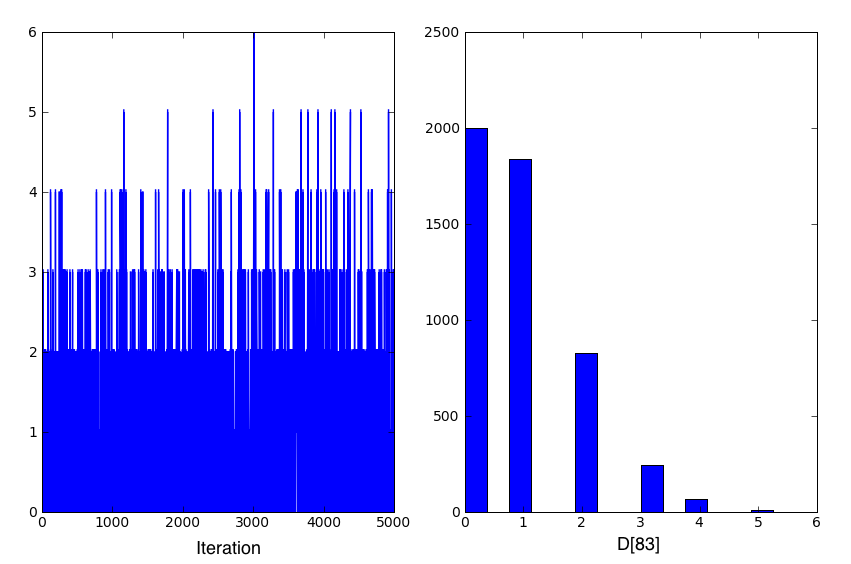
\includegraphics[height=3in]{missing.png}
\caption{Trace and posterior distribution of the second missing data point in the example.}
\label{fig:missing}
\end{center}
\end{figure}

The main limitation of this approach for imputation is performance. Because each element in the data array is modelled by an individual Stochastic, rather than a single Stochastic for the entire array, the number of nodes in the overall model increases from 4 to 113. This significantly slows the rate of sampling, since the model iterates over each node at every iteration.

% section missing_data (end)